\section{Analyse des Schaltplans vom Empfänger} %Erik

\section{Vorverstärkung des Signals} %Lukas
\subsection{Friis-Formel}
Die Friis-Formel ist ein wichtige Formel in der Nachrichtentechnik um die Rauschzahl SNR einer Kette von Verstärkern
bzw. Dämpfungsgliedern zu berechnen.

\begin{figure}[H]
    \centering
    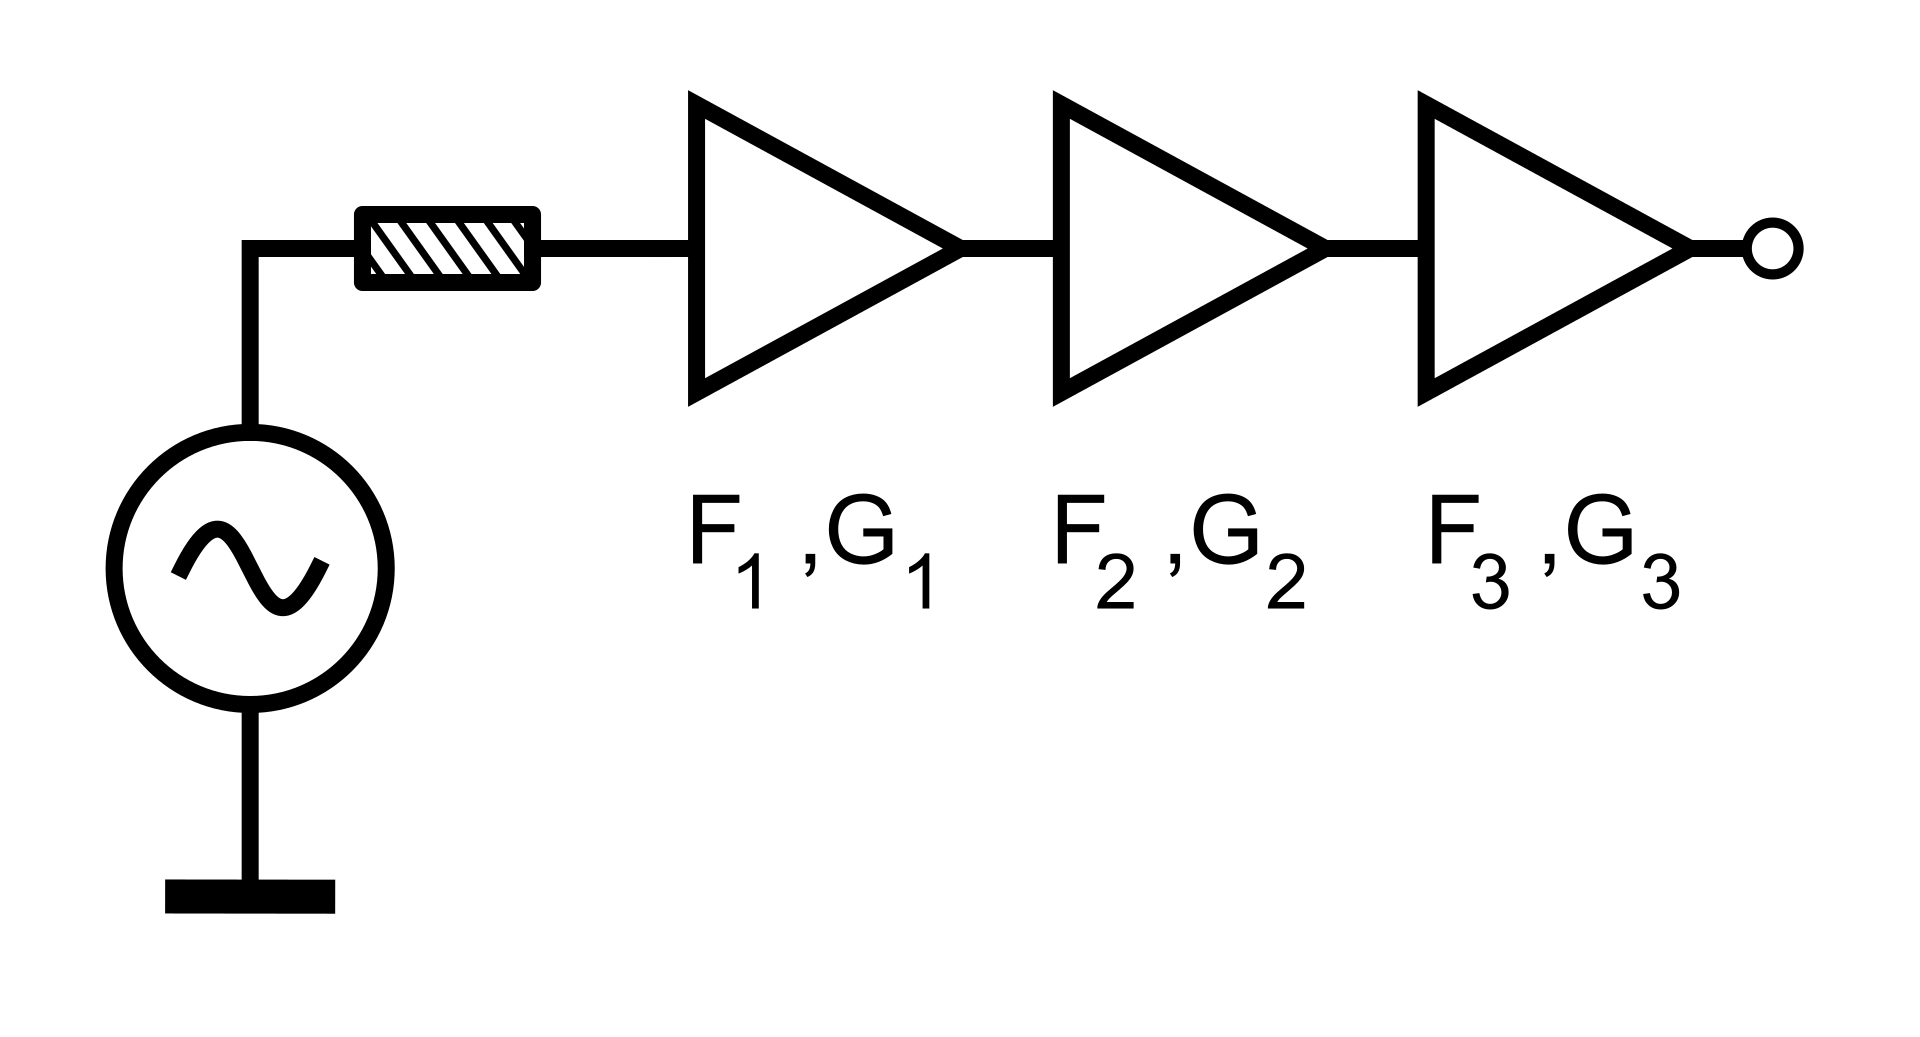
\includegraphics[width=0.5\textwidth]{Pictures/Frijs-Kette.svg.png}
    \caption{Verstärkerkette}
    \footnotesize{Quelle: \url{https://de.wikipedia.org/wiki/Friis-Formel#/media/Datei:Frijs-Kette.svg}}
    %\label{fig:link_budget}
\end{figure}
Für eine Verstärkerkette mit $n$ Verstärkern ergibt sich die Rauschzahl folgendermaßen:
\begin{equation}
    F_{\text{gesamt}} = 1 + (F_1 - 1) + \frac{F_2 - 1}{G_1} + \frac{F_3 - 1}{G_1 G_2} + \frac{F_4 - 1}{G_1 G_2 G_3} + \dots + \frac{F_n - 1}{G_1 G_2 G_3 \dots G_{n-1}}
\end{equation}
\begin{itemize}
    \item $F_{\text{gesamt}}$: Die Gesamte Rauschzahl der Verstärkerkette
    \item $F_i$: Die Rauschzahl des $i$-ten Verstärkers
    \item $G_i$: Die Verstärkung des $i$-ten Verstärkers
\end{itemize}
Es wird schnell ersichtlich, dass Verstärker am Anfang der Kette, am meisten Einfluss auf die Gesamtrauschzahl haben.
Deswegen sollten die Verstärker mit dem höchsten Gewinn immer am Anfang der Kette stehen. Andersherum sollten Bauteile mit Dämpfung am Ende der Kette stehen.
\\
Deshalb sollte ein Signal immer zuerst vorverstärkt werden, bevor die Frequenzkonversion durchgeführt wird.
Würde das Signal zuerst gemischt und dann Nachverstärkt werden, hätten wir im Vergleich ein deutlich höheres Rauschen.
Da der Verstärker im Vergleich zum Mischer ein höheren Gewinn hat, je nach Mischer kann dieser sogar auch dämpfend wirken.
\section{Frequenz-Downkonversion} %Farhad
\subsection{Ablauf der Frequenz-Downkonversion in der Schaltung}
\subsection{Funktion des Widerstandes R\textsubscript{24}}

\section{Operationsverstärkerschaltung} %Lukas 5a und c

\section{Komparatorschaltung} %Erik 6 a und b
\clearpage